\documentclass{article}
\usepackage{titling}          % For å legge til undertittel
\usepackage{fontawesome5}      % For GitHub-symbolet
\usepackage{hyperref} 
\usepackage{graphicx} % Required for inserting images
\usepackage[utf8]{inputenc}
\usepackage[T1]{fontenc}
\usepackage{lmodern}
\usepackage[scaled]{beramono}
\usepackage[final]{microtype}
\usepackage{amssymb}
\usepackage{mathtools}
\usepackage{tikz}
\usepackage{algorithm}
\usepackage[noend]{algpseudocode}
\usepackage{amsmath}
\usepackage{bm}
\usepackage{tcolorbox}
\usepackage{hyperref}
\usepackage{multicol}
\setlength{\columnsep}{0.5cm} % Setter spalteavstand til 1 cm
\usepackage{amsthm}
\usepackage{thmtools}
\usepackage{babel}
\usepackage{caption}
\captionsetup[figure]{labelfont=bf, font=small}  % Setter "Figure X" i bold og tekst i liten skrift
\usepackage{titlesec} % For å tilpasse seksjon- og underseksjonsoverskrifter
\usepackage{textcase} % For å automatisk konvertere til caps

\usepackage{csquotes}
\usepackage{listings}
\lstset{basicstyle = \ttfamily}
\usepackage{textcomp}
\usepackage{siunitx}
\usepackage{xcolor}
\usepackage{tikz}
\usetikzlibrary{positioning}
\usepackage{graphicx}
\usepackage{float}
\usepackage{matlab-prettifier}
\usepackage[colorlinks, allcolors = uiolink]{hyperref}
\usepackage[a4paper, left=3.5cm, right=3.5cm, top=2.5cm, bottom=2.5cm]{geometry}

\newcommand{\EE}{\mathbb{E}}
\newcommand{\bb}[1]{\boldsymbol{#1}}
\newcommand{\ty}{\tilde{\bb{z}}}
\newcommand{\XX}{\mathbf{X}} 
\newcommand{\VV}{\mathbf{V}} 
\newcommand{\UU}{\mathbf{U}} 
\newcommand{\SS}{\mathbf{\Sigma}}

% Format for seksjonsoverskrifter
\titleformat{\section}
  {\centering\bfseries\MakeTextUppercase} % Midtstilt, bold, caps
  {\thesection}{1em}{} % Nummereringsformatet for seksjon

% Format for underseksjonsoverskrifter (venstrestilt, bold, samme størrelse som brødtekst)
\titleformat{\subsection}
  {\bfseries} % Bold, samme størrelse som brødtekst (12pt)
  {\thesubsection}{1em}{} % Nummereringsformatet for subseksjon

% Format for underseksjonsoverskrifter (venstrestilt, bold, samme størrelse som brødtekst)
\titleformat{\subsubsection}
  {\bfseries} % Bold, samme størrelse som brødtekst (12pt)
  {\thesubsection}{1em}{} % Nummereringsformatet for subseksjon

\setlength{\parskip}{0pt} % Fjerner mellomrom mellom avsnitt
\setlength{\parindent}{15pt} % Beholder innrykk

% Fjerne ekstra mellomrom mellom underseksjon og tekst
\titlespacing{\subsection}{0pt}{*1}{*0} % Ingen vertikal plass før eller etter subsection
\titlespacing{\subsubsection}{0pt}{*1}{*0} % Ingen vertikal plass før eller etter subsection

%%%%%%%%%%%%%%%%%%%%%%%%%%%%%%%%%%%%%%%%%%%%%%%%%%%%%%%%
%                   TITTEL/CREDITS                     %
%%%%%%%%%%%%%%%%%%%%%%%%%%%%%%%%%%%%%%%%%%%%%%%%%%%%%%%%

\title{FYS-STK3155: Regression Analysis and Resampling Techniques in Applied Machine Learning}

\author{Oscar Atle Brovold, Eskil Grinaker Hansen, Håkon Ganes Kornstad}
\date{October 7, 2024}

\begin{document}
\maketitle
\begin{center}
    \href{https://github.com/EOH-ML/FYS-STK3155-Projects/tree/main/project1}{\texttt{Project GitHub Repository}}
\end{center}

%%%%%%%%%%%%%%%%%%%%%%%%%%%%%%%%%%%%%%%%%%%%%%%%%%%%%%%%
%                   ABSTRACT/INTRO                     %
%%%%%%%%%%%%%%%%%%%%%%%%%%%%%%%%%%%%%%%%%%%%%%%%%%%%%%%%

\begin{abstract}
\noindent In this paper, we analyze three different methods for polynomial regression in machine learning: Ordinary Least Squares, Ridge, and Lasso Regression. We evaluate their performance with mean squared error and R$^2$-score, and we explore data resampling techniques such as bootstrapping and \textit{k}-fold cross validation. First we fit the models to a two dimensional test function, and then to real mountain data from Norway. We find the Ordinary Least Squares to outperform both Ridge and Lasso in approximating real landscapes.
\end{abstract}
\vspace{15pt}
\begin{multicols}{2}
\vspace{0pt}
\section*{INTRODUCTION} 
With an ever growing wealth of data, and the computational power to match it, machine learning is a rapidly growing field. It is now being used across a wide array of domains, including finance, physics and healthcare \cite{sarker_machine_2021}. Its methods can provide us with insight into dimensions beyond human comprehension.

One of the most fundamental principles of machine learning is the use of regression methods \cite{hastie_elements_2009}, employed for either prediction or classification. In this paper, we will investigate three basic methods of \textit{linear} regression: Ordinary Least Squares (OLS), Ridge, and Lasso. First, we apply these regression methods to data generated by the continuous Franke’s Function\cite{franke_critical_1975}, both with and without noise. To improve the models’ performance, we apply oversampling techniques such as bootstrapping and \textit{k}-fold cross validation. Hyperparameters, such as the degree of complexity and the regularization term $\lambda$, are then fine-tuned to improve the models’ fit to the data. We evaluate and compare the accuracy of each model using statistics such as Mean Squared Error (MSE) and R$^2$-scores.

Finally, we extend this analysis to real terrain data from Evja outside of Stavanger, Norway, applying the same methods.

%%%%%%%%%%%%%%%%%%%%%%%%%%%%%%%%%%%%%%%%%%%%%%%%%%%%%%%%
%                       TEORI                          %
%%%%%%%%%%%%%%%%%%%%%%%%%%%%%%%%%%%%%%%%%%%%%%%%%%%%%%%%

\section*{Theoretical background}
\textbf{Note:} If no other sources are referenced, the theoretical part is based on the course lecture notes. \cite{hjorth-jensen_applied_2021}

\subsection*{Regression Analysis}
\begin{figure}[H]
    \centering
\includegraphics[width=\columnwidth]{figures/ols_ill.eps}
    \caption{All regression problems in $\mathbb{R}$ involve fitting a line to a set of points, and measuring the errors. This problem can be generalized to higher dimensions, fitting a hyperplane in $\mathbb{R}^n$}
    \label{fig:ols_illustration}
\end{figure}
Given a dataset, we assume that the observations $\bm{z}$ are generated by the following equation
\begin{equation} \label{eq:given data}
\bm{z} = f(\mathbf{x}) + \boldsymbol{\varepsilon}
\end{equation}
where $\bm{z}$ represent the observed responses, $f(\bm{x})$ is an unknown, non-stocahastic function, and $\bm{\varepsilon}$ is stochastic noise. The objective of regression is to approximate $f(\bm{x})$ using the observed data. (For more details, appendix \ref{app_derivations:expectation_variance_true_z})

To achive this we optimize a set of coefficients $\hat{\boldsymbol{\beta}}$ and predict with the following equation
$$\bm{\tilde{z}} = \mathbf{X} \hat{\boldsymbol{\beta}}$$
Here $\bm{\tilde{z}}$ is the predicted responses and $\mathbf{X}$ is the \textit{design matrix}. In $\mathbf{X}$, each column represents a feature, and the rows represent samples.

By applying a polynomial transformation to the input data, we can capture the polynomial relationship between the input and output while maintaining a linear framework. This approach is commonly known as polynomial regression. To capture these features, the Vandermonde matrix \cite{weisstein_vandermonde_nodate} is commonly used:
$$\mathbf{X} = \begin{pmatrix}
    1 & x_1 & x_1^2 & \cdots & x_1^{p-1} \\
    1 & x_2 & x_2^2 & \cdots & x_2^{p-1} \\
    \vdots & \vdots & \vdots & \ddots & \vdots \\
    1 & x_{n-1} & x_{n-1}^2 & \cdots & x_{n-1}^{p-1}
\end{pmatrix}$$
When given two input sets $\bm{x}$ and $\bm{y}$, the permutations for each column is given as all combinations $x_i^ay_j^b$ where $a + b \leq p-1$. The total number of such combinations, i.e terms in the polynomial, is given by the expression 
$$ \text{N} = \frac{(p + 1)(p+2)}{2} $$ 

\subsubsection*{Ordinary Least Squares}
Our goal is to calculate the linear model that best fits or approximates the data in equation \ref{eq:given data}. In the case of OLS the cost function is given by:

\begin{equation} \label{eq:cost ols}
    C_{\text{OLS}}(\boldsymbol{\beta}) = \|\bm{z} - \mathbf{X} \bm{\beta}\|_2^2
\end{equation}
We aim to find the coefficients $\hat{\boldsymbol{\beta}}$ that minimizes \ref{eq:cost ols}. This can be done by differentiating with respect to $\bm{\beta}$ and set it equal to zero:
$$ \frac{\partial}{\partial \bm{\beta}} \|\bm{z} - \mathbf{X} \boldsymbol{\beta}\|_2^2 = 0 $$
This can be shown to lead to the \textbf{normal equation} (See appendix \ref{app_derivations:beta_ols_without_svd} for full derivation):
$$ \hat{\boldsymbol{\beta}}_{OLS} = \left( \mathbf{X}^\top \mathbf{X} \right)^{-1} \mathbf{X}^\top \bm{z} $$

The solution assumes that $\mathbf{X}^\top \mathbf{X}$ is invertible, which holds when $\mathbf{X}$ has full column rank \cite{guntuboyina_fall_nodate}. If $\mathbf{X}^\top \mathbf{X}$ is not invertible (singular), alternative methods such as regularization or using a pseudoinverse can be applied.\cite{deisenroth_mathematics_2020}

% Ta med bevis for OLS med Varians
\subsubsection*{Ridge Regression}
 Ridge regression expands on OLS to prevent overfitting and manage multicollinearity. This is done by adding a regularization term $\lambda \| \bm{\beta} \|_{2}^{2}$ to the OLS cost function \cite{noauthor_what_2023}, leading to
\begin{align} \label{eq:rigde cost}
C_{\text{Ridge}}(\mathbf{X}, \bm{\beta}) = \| \mathbf{X} \bm{\beta} - \bm{z} \|_2^2 + \lambda \| \bm{\beta} \|_{2}^{2}
\end{align}
The regularization term introduces a constraint that penalizes larger coefficient values. The degree of this regularization is then controlled by the parameter $\lambda$. 
As $\lambda \rightarrow 0$, Ridge regression behaves like OLS. As $\lambda$ increases, the regularization effect grows, thus shrinking the coefficients more.

When minimizing \ref{eq:rigde cost} with respect to $\bm{\beta}$, we get the optimal coefficients (See appendix \ref{app_derivations:beta_ridge_without_svd} for full derivation):
$$\bm{\hat{\beta}}_{\text{Ridge}} = (\mathbf{X}^\top \mathbf{X} + \lambda\mathbf{I})^{-1}\mathbf{X}^\top \bm{z}$$ 
Ridge regression mitigates the issue of $\mathbf{X}^\top \mathbf{X}$ being singular or near singular (ill-conditioned), by replacing it with $\mathbf{X}^\top \mathbf{X} + \lambda\mathbf{I}$, which is always invertible, leading to stabler coefficient estimates.
\cite{deisenroth_mathematics_2020}

\subsubsection*{Lasso Regression}
Similar to Ridge regression, Lasso regression  introduces a regularization term, but instead of the L2-norm, it uses the L1-norm, defined as $\lambda \| \bm{\beta} \|_{1}$ \cite{tibshirani_regression_1996}. This results in the following cost function:
\begin{equation} \label{eq:lasso cost}
    C_{\text{Lasso}}(\mathbf{X}, \bm{\beta}) = \| \mathbf{X} \bm{\beta} - \bm{z} \|_2^2 + \lambda \| \bm{\beta} \|_{1}
\end{equation}
The key difference in Ridge and Lasso regression lies in the nature of their regularization. While Ridge regression shrinks the coefficients towards zero, Lasso regression can set specific coefficients \textit{exactly} to zero. This property makes Lasso useful in feature selection, effectively eliminating less important features. The resulting model is simpler and more interpretable, especially in high-dimensional datasets with feature dependencies.

As with OLS and Ridge, the goal in Lasso is to minimize the cost function \ref{eq:lasso cost} to find the optimal coefficients:
$$\bm{\hat{\beta}} = \arg \min_{\bm{\beta}} \left( \| \mathbf{X} \bm{\beta} - \bm{y} \|_2^2 + \lambda \| \bm{\beta} \|_1 \right)$$
However, unlike OLS and Ridge, this expression does give us an analytic expression, and must be computed using optimization techniques \cite{gauraha_introduction_2018}.

\begin{figure}[H]
    \centering
    \includegraphics[width=\columnwidth]{figures/ridge_lasso.eps}
    \caption{Comparison of the effect of regularization in Lasso and Ridge regression. Lasso uses the L1-norm, which can shrink some coefficients to zero, leading to feature selection. Ridge uses the L2-norm, shrinking all coefficients but retaining non-zero values, which helps manage multicollinearity without feature elimination.}
    \label{fig:ridge_lasso}
\end{figure}

\subsubsection*{Singular Value Decomposition}
When $\mathbf{X}^\top\mathbf{X}$ is singular or ill-conditoned, using the psuedoinverse can provide a more stable optimization. This is where the singular value decomposition (SVD) is useful. For any $n \times m$ matrix $\mathbf{A}$, the SVD is given by:
$$\mathbf{A} = \mathbf{U}\mathbf{\Sigma}\mathbf{V^\top}$$
where $\mathbf{U}$ and $\mathbf{V}$ are orthonormal matrices, and $\mathbf{\Sigma}$ is a diagonal matrix containing the singular values.\cite{lay_linear_2016}

The pseudoinverse of $\mathbf{A}$ can be performed by taking the pseudoinverse of $\mathbf{\Sigma}$ only. This involves flipping its dimensions and replacing every nonzero entry $\sigma_i$
with $\frac{1}{\sigma_i}$

The pseudoinverse allows us to compute the coefficients for OLS as: 
$$ \hat{\bm{\beta}}_\text{OLS} = 
\mathbf{V}(\mathbf{\Sigma}^\top\mathbf{\Sigma})^{+}\mathbf{\Sigma}^\top\mathbf{U}^\top\bm{y} $$
Equally, we can obtain the coefficients for Ridge:
$$ \hat{\bm{\beta}}_\text{Ridge} = 
\mathbf{V}(\mathbf{\Sigma}^\top\mathbf{\Sigma} + \lambda\mathbf{I})^{+}\mathbf{\Sigma}^\top\mathbf{U}^\top\bm{y} $$
(For full derivations see appendix \ref{app_derivations:beta_ols_with_svd} and \ref{app_derivations:beta_ridge_with_svd})

\section*{Data}
\subsubsection*{Franke's function} 

\begin{align*}
f(x, y) &= \frac{3}{4} \exp\left(-\frac{(9x - 2)^2}{4} - \frac{(9y - 2)^2}{4}\right)\\ 
&+ \frac{3}{4} \exp\left(-\frac{(9x + 1)^2}{49} - \frac{(9y + 1)}{10}\right)\\
&+ \frac{1}{2} \exp\left(-\frac{(9x - 7)^2}{4} - \frac{(9y - 3)^2}{4}\right)\\ 
&- \frac{1}{5} \exp\left(-(9x - 4)^2 - (9y - 7)^2\right)
\end{align*}
This bivariate function by R. Franke (1975) \cite{franke_critical_1975} is given by the weighted sum of four exponentials, and it generates terrain-like data (see figure \hyperref[fig:F1]{\textbf{F1}} and \hyperref[fig:F1]{\textbf{F2}}). It is well-suited for testing interpolation, regression, and surface-fitting algorithms because of its continuous quality, with a varying curvature.

\subsubsection*{Terrain Data} 
The real world terrain data for this project is provided by the U.S. Department of the Interior Geological Surveys (USGS) EarthExplorer website \cite{earth_resources_observation_and_science_eros_center_shuttle_2017}. The area of interest in our analysis is from Evje outside Stavanger.

\subsubsection*{Splitting the Data}
Generally, in machine learning, we split the data into a \texttt{training\_set} and a \texttt{test\_set} before training the model. This is often done with a ratio of 80:20 in favor of the training set. \cite{joseph_optimal_2022}

\subsubsection*{Bootstrapping}
The bootstrap method is a resampling technique in which samples are repeatedly drawn from a dataset with replacement, effectively generating multiple resampled datasets. The method is non-parametric, meaning it does not assume any distribution, making it a highly versatile method for model evaluation and performance estimation.

When evaluating statistics, there may be some uncertainty in the estimates. By using the bootstrap method, we are likely to obtain a more representative estimate of the given statistic. \cite{storvik_bootstrapping_nodate}
(See appendix \ref{app_resamp:bootstrap} for the bootstrap algorithm)

\subsubsection*{\textit{k}-fold Cross Validation}
In \textit{k}-fold cross validation, the \texttt{training\_set} is split into $k$ non-overlapping subsets, or \textit{folds}. For each of the $k$ iterations, one fold is used as the \texttt{validation\_set} (also referred to as the \texttt{test\_set}), while the remaining $(k-1)$ folds are used to train the model. This process is repeated until every fold has been used for validation. After all $k$ iterations, the performance of the model can be evaluated by calculating the average of a chosen statistic from each fold's result (see Figure \ref{fig:cross_validation}). %(source ellis here)

\begin{figure}[H]
    \centering
    \includegraphics[width=\columnwidth]{figures/cross_validation_alt.eps}
    \caption{\textit{k}-fold cross validation, where the average statistic can be calculated as $\frac{1}{k}\sum_{i=0}^{k-1} \hat{\theta}_i$.}
    \label{fig:cross_validation}
\end{figure}

\subsection*{Quantification methods}
\subsubsection*{Mean squared error}
A common way to quantify the error, is a statistic known as the mean squared error, which is given by
$$\text{MSE} = \frac{1}{n} \sum_{i=0}^{n-1}(z_i - \tilde{z}_i)^2 = \EE[(\bm{z} - \bm{\tilde{z}})^2]$$
It quantifies the average squared difference between the true response $\bm{z}$ and the predicted response $\bm{\tilde{z}}$. The MSE can be further understood by a decomposition into a variance term and a bias term. The decomposistion is given by: 
\begin{equation} \label{eq:mse,bias-var}
  \EE[(\mathbf{y} - \mathbf{\tilde{y}})^2] = \text{Bias}[\mathbf{\tilde{y}}] + \text{Var}[\mathbf{\tilde{y}}] + \sigma^2  
\end{equation}
(See appendix \ref{app_derivations:bias_variance_decomp} for full derivation)

\subsubsection*{Bias-Variance Tradeoff} As shown in equation \ref{eq:mse,bias-var}, the MSE can be decomposed into bias and variance. \textbf{Bias} reflects how consistently a model deviates from the true data, while \textbf{variance} measures the model’s sensitivity to fluctuations in the training data. 
We aim for our model to have both low bias and low variance, however this balance is difficult to obtain, hence the \textbf{bias-variance tradeoff}. As model complexity increases, bias typically decreases and variance tends to rise. A less complex model might achieve a better balance, which can result in not selecting the model with the lowest MSE.

If we select a model with high bias, its ability to capture the underlying patterns in the data is weakened. This often results in low variance, as the model struggles to adjust to the complexity. This phenomenon is known as \textbf{underfitting}. Conversely, \textbf{overfitting} is often a result of high variance. This is where the model is to flexible and captures too much of the noise in the data. 

\subsection*{Expectation and variance of OLS coefficients}
We can further explore the behaviour of the optimal coefficients for OLS by analyzing the estimator's properties. The expectation of $\bm{\hat{\beta}}$ is:
$$\EE[{\bm{\hat{\beta}}}] = \bm{\beta}$$
This shows that the OLS estimator is unbiased. It is however important to note that unbiasedness does not imply low variance. The variance for OLS is given by:
$$\text{Var}[\bm{\hat{\beta}}] = \sigma^2(\mathbf{X}^\top\mathbf{X})^{-1}$$
(See appendix \ref{app_derivations:expectation_variance_betas} for full derivation) It can therefore sometimes be useful to include a regularization to make the estimator biased, but reduce the variance.

It is now possible to derive a 95$\%$ confidence interval (CI) for each $\beta_j$, given as:
\begin{equation} \label{eq:CI}
    CI = \beta_j \pm 1.96\sigma^2(\beta_j)
\end{equation}
This interval gives a range in which we expect the true $\beta_j$ to lie with $95\%$ confidence.

\subsection*{The $\mathbf{R^2}$-score}
Another statistic used to quantify the model’s performance is the $R^2$-score. This statistic provides a measure of how well the model predicts unseen data, and is defined as:
$$R^2(\bm{z}, \bm{\tilde{z}}) = 1 - \frac{\sum_{i=0}^{n-1} (z_i - \hat{z}_i)^2}{\sum_{i=0}^{n-1} (z_i - \bar{z})^2}$$
The score is typically in the range $[0,1]$, where $1$ indicates a perfect fit, meaning that the model explains all variance in the data. In particular, if our score is $r$, we can interpret this as our model accounting for $r\times100\%$ of the variance in the data. 
\end{multicols}
\newpage

%%%%%%%%%%%%%%%%%%%%%%%%%%%%%%%%%%%%%%%%%%%%%%%%%%%%%%%%
%                       FRANKE                         %
%%%%%%%%%%%%%%%%%%%%%%%%%%%%%%%%%%%%%%%%%%%%%%%%%%%%%%%%

\section*{Initial Testing with Franke’s function}
\begin{multicols}{2}
We begin by generating data from Franke’s function, and plotting it (\hyperref[fig:F1]{\textbf{F1}}, \hyperref[fig:F1]{\textbf{F2}}). F1 is the continous Franke's funtion, and F2 is Franke's function with a regu larized Gaussian noise, given by: 
$$f_{\text{Franke}}(\bm{x}) + \eta \cdot \mathcal{N}(0, 1)$$
The plots show that it generates synthesized terrain-data, which would be meaningful to use for testing.
We create the design matrix (Appendix \ref{app_alg:design_matrix}), split the data into a \texttt{training\_set} and \texttt{test\_set} using \texttt{train\_test\_split()} from \texttt{scikit learn} \cite{pedregosa_et_al_scikit-learn_2011}, before scaling the data. 

\begin{tcolorbox}[colback=gray!10, colframe=gray!10]
We use \textbf{subtract mean} scaling throughout this project: Each feature is centered by subtracting the mean of its column, but no further scaling by standard deviation is applied. This ensures that all features are centered, without altering their original variance. It also prevents any feature from dominating the model and maintains the data (i.e. the terrain's original curvature), by retaining its natural variability.
\end{tcolorbox}

We now apply scaling on our training data, \texttt{X\_train}, using subtract mean scaling to center each feature around zero. Similarly, \texttt{z\_train} is centered by subtracting its mean, ensuring that the target values are also zero-centered. To maintain consistency between training and testing, the test data, \texttt{X\_test}, is scaled using the mean values computed from the training data. This ensures that the test data is scaled in the same way as the training set.

Furthermore, in our analysis we use $\texttt{intercept} = \texttt{False}$, meaning that the intercept is included in the design matrix, rather than being calculated separately after training (See appendix \ref{app_prep:intercept} for detailis). We test with Franke's function and find that the choice has a negligible impact on model performance, so we adopt this as a default for all regression models from now on.

\subsubsection*{Method of Inversion: SVD} 
To ensure stability in our regression methods (OLS and Ridge), we need a robust approach for computing the inverse when the matrices are singular or ill-conditioned. From the theory section on 
SVD, we know that SVD can be used to compute a pseudoinverse. In figure \hyperref[fig:F3]{\textbf{F3}}, we compare the performance of using the pseudoinverse and the standard matrix inverse for OLS. From polynomial degree 9 onward, SVD stabilizes the OLS method, whereas standard inversion leads to instability. Therefore, we employ SVD as a default for matrix inversion. 

\subsubsection*{Tuning the Noise Parameter $\eta$} To mimic real terrain with Franke's function, we need to find a noise term $\eta$ that best replicates the variations in a natural landscape. We can observe that as $\eta \rightarrow 0$, OLS outperforms L2-norm regularization. On the other hand, if $\eta$ is increased, more regularization shows improvement in MSE. If we want Franke's function to mimic a real terrain we need a sweetspot for $\eta$. If $\eta$ is too large, the terrain becomes unrealisticly noisy; if $\eta$ is too small, the terrain becomes too smooth. Based on our observations, we propose that $\eta = 0.1$ could be our sweetspot. We will use this value when further analysing Franke's function. 

\section*{Performance evaluation of Franke’s Function}
Having established our fundamental methods, we are now prepared to conduct model analysis on Franke's function. We begin with $k$-fold cross validation which will help identifying the model that performs best with respect to the MSE.

To further evaluate the models, we employ the bootstrap method in conjunction with a bias-variance tradeoff analysis. This approach will deepen our understanding of the models' stability and generalization capabilities across different datasets.

\subsubsection*{Using $k$-fold cross validation}
Before determining which hyperparameters yield the best model, we need to select an appropriate value for $k$.  
The choice of $k$ is partly arbritrary, however $k = 10$ is often regarded as the best practice. It provides stable estimates of error (See figure \hyperref[fig:F4]{\textbf{F4}}) without excessive computational expense. %source (ellis?)

With the cross-validation framework established, we proceed to tuning of the hyperparameters $\lambda$ and degree of complexity. We test the following values for $\lambda$: 
$$\lambda \in \{\,0\,\} \cup \{ 10^{k} \;\big|\; k \in \{-9, -8, \ldots, 1\} \}$$
where $\lambda = 0$ corresponds to the OLS solution, and 
$\text{complexity} \in \{0, 1, \ldots, 20\}$.
For each combination of $\lambda$ and complexity we apply cross-validation to obtain more accurate estimates of the MSE-values. 

The resulting MSE-values are visualized in a heatmap (see figures \hyperref[fig:F6]{\textbf{F6}}, \hyperref[fig:F7]{\textbf{F7}}), with $\lambda$ along the x-axis and complexity along the y-axis. The left plot corresponds to Ridge regression (with OLS included at $\lambda = 0$) and the right corresponds to Lasso regression. In both plots we have highlighted the combination yielding the minimal MSE-value. 

The plot for Ridge and OLS shows that $\text{complexity} = 18$ and $\lambda = 10^{-9}$ result in a minimal $\text{MSE} = 0.01034$. Lasso regression performs worse than both Ridge and OLS, with a minimal $\text{MSE} = 0.01433$ for $\text{complexity} = 18$ and $\lambda = 10^{-7}$. This suggests that the L2-norm regularization could be benefical in estimating Franke's function. On the other hand, the L1-norm regularization appears to be less effective.

\subsubsection*{Applying bootstrap for bias-variance analysis}
To further analyze the data, we employ the bootstrap method. We implement bootstrap resampling with OLS, exploring model complexity $\in \{1, 2, \ldots, 25\}$. Specifically, we use it to derive a bias-variance tradeoff analysis. 

From figure \hyperref[fig:F8]{\textbf{F8}} we can see that the MSE and bias decreases significantly within the first four degrees of complexity. However, after degree four, the values stabilize, with the MSE showing a slight increase starting around degree 18.

It is important to also take the variance into consideration. For lower complexities the variance is close to zero, however it increases rapidly as the the model gets more complex. This rise in variance highlights the danger of overfitting with more complex models. 

From a visual inspection, it seems that the optimal tradeoff lies within polynomial degree seven and ten.

\subsubsection*{Analysis of the optimized coefficients}%eskil
The way we set up the design matrix has some unfortunate effects on the analysis of the coefficients. Specifically, we will not obtain the same $\beta_i$ for a given permutation of $x$ and $y$ across models with different complexities. However, the plot will still be meaningful for a general analysis, as we can observe the overall tendencies in bias and variance.

As stated in theory section we can estimate the coefficients along with their confidence intervals. This could improve our understanding of the bias-variance tradeoff. As shown in figure \hyperref[fig:F5]{\textbf{F5}}, the spread of each coefficient-estimate ($\beta_i$) increases as model complexity grows, reflecting higher variance. Furthermore, analysis of each $\beta_i$ within the same model complexity shows that increased complexities yield more spread, hence lower bias. This supports our bias-variance reasoning. 

\subsection*{A note on the R$^2$-score}
We will now use the R$^2$-score to verify our results. As discussed in the theoretical section, it provides a measure of how much of the variability in the data we are able to capture. From Figure \hyperref[fig:F9]{\textbf{F9}}, we can see that both OLS and Ridge regression achieve stable and high R$^2$-scores (around $90\%$).

In contrast, Lasso regression performs worse, as also observed in the MSE analysis. This suggests that Lasso struggles to capture the variability effectively. Most likely due to how it handles sparsity in the model coefficients. 

\subsubsection*{Concluding the initial testing}
We now need to take all of our analysis into consideration: From the k-fold cross validation analysis, we find the best hyperparameters and model to minimize the MSE to be Ridge regression with regularization term $\lambda=10^{-9}$ and complexity 18.

However, to perform regression on an arbitrary new set of data, a small MSE can not be the only component to determine the best-fitting model. Therefore we also take a look at the bias-variance analysis. This method of analysis favours smaller complexities, where the best tradeoff lies in the range of complexity seven to ten.

With this knowledge we are ready to test our methods on real terrain data.
\end{multicols}

\begin{figure}[H]
    \centering
    \fbox{
    \begin{minipage}{\textwidth}
        \centering
        \begin{minipage}{0.32\textwidth}
            \centering
            \textbf{F1} \label{fig:F1} \\  % Label added
            \includegraphics[width=\textwidth]{figures/hakon/franke_min.png}
        \end{minipage}
        \hfill
        \begin{minipage}{0.32\textwidth}
            \centering
            \textbf{F2} \label{fig:F2} \\  % Label added
            \includegraphics[width=\textwidth]{figures/hakon/franke_min_noise.png}
        \end{minipage}
        \begin{minipage}{0.34\textwidth}
            \centering
            \textbf{F3} \label{fig:F3} \\  % Label added
            \includegraphics[width=\textwidth]{figures/hakon/svd_ols_minimal.png}
        \end{minipage}
        \begin{minipage}{0.64\textwidth}
            \centering
            \textbf{F4} \label{fig:F4} \\  % Label added
            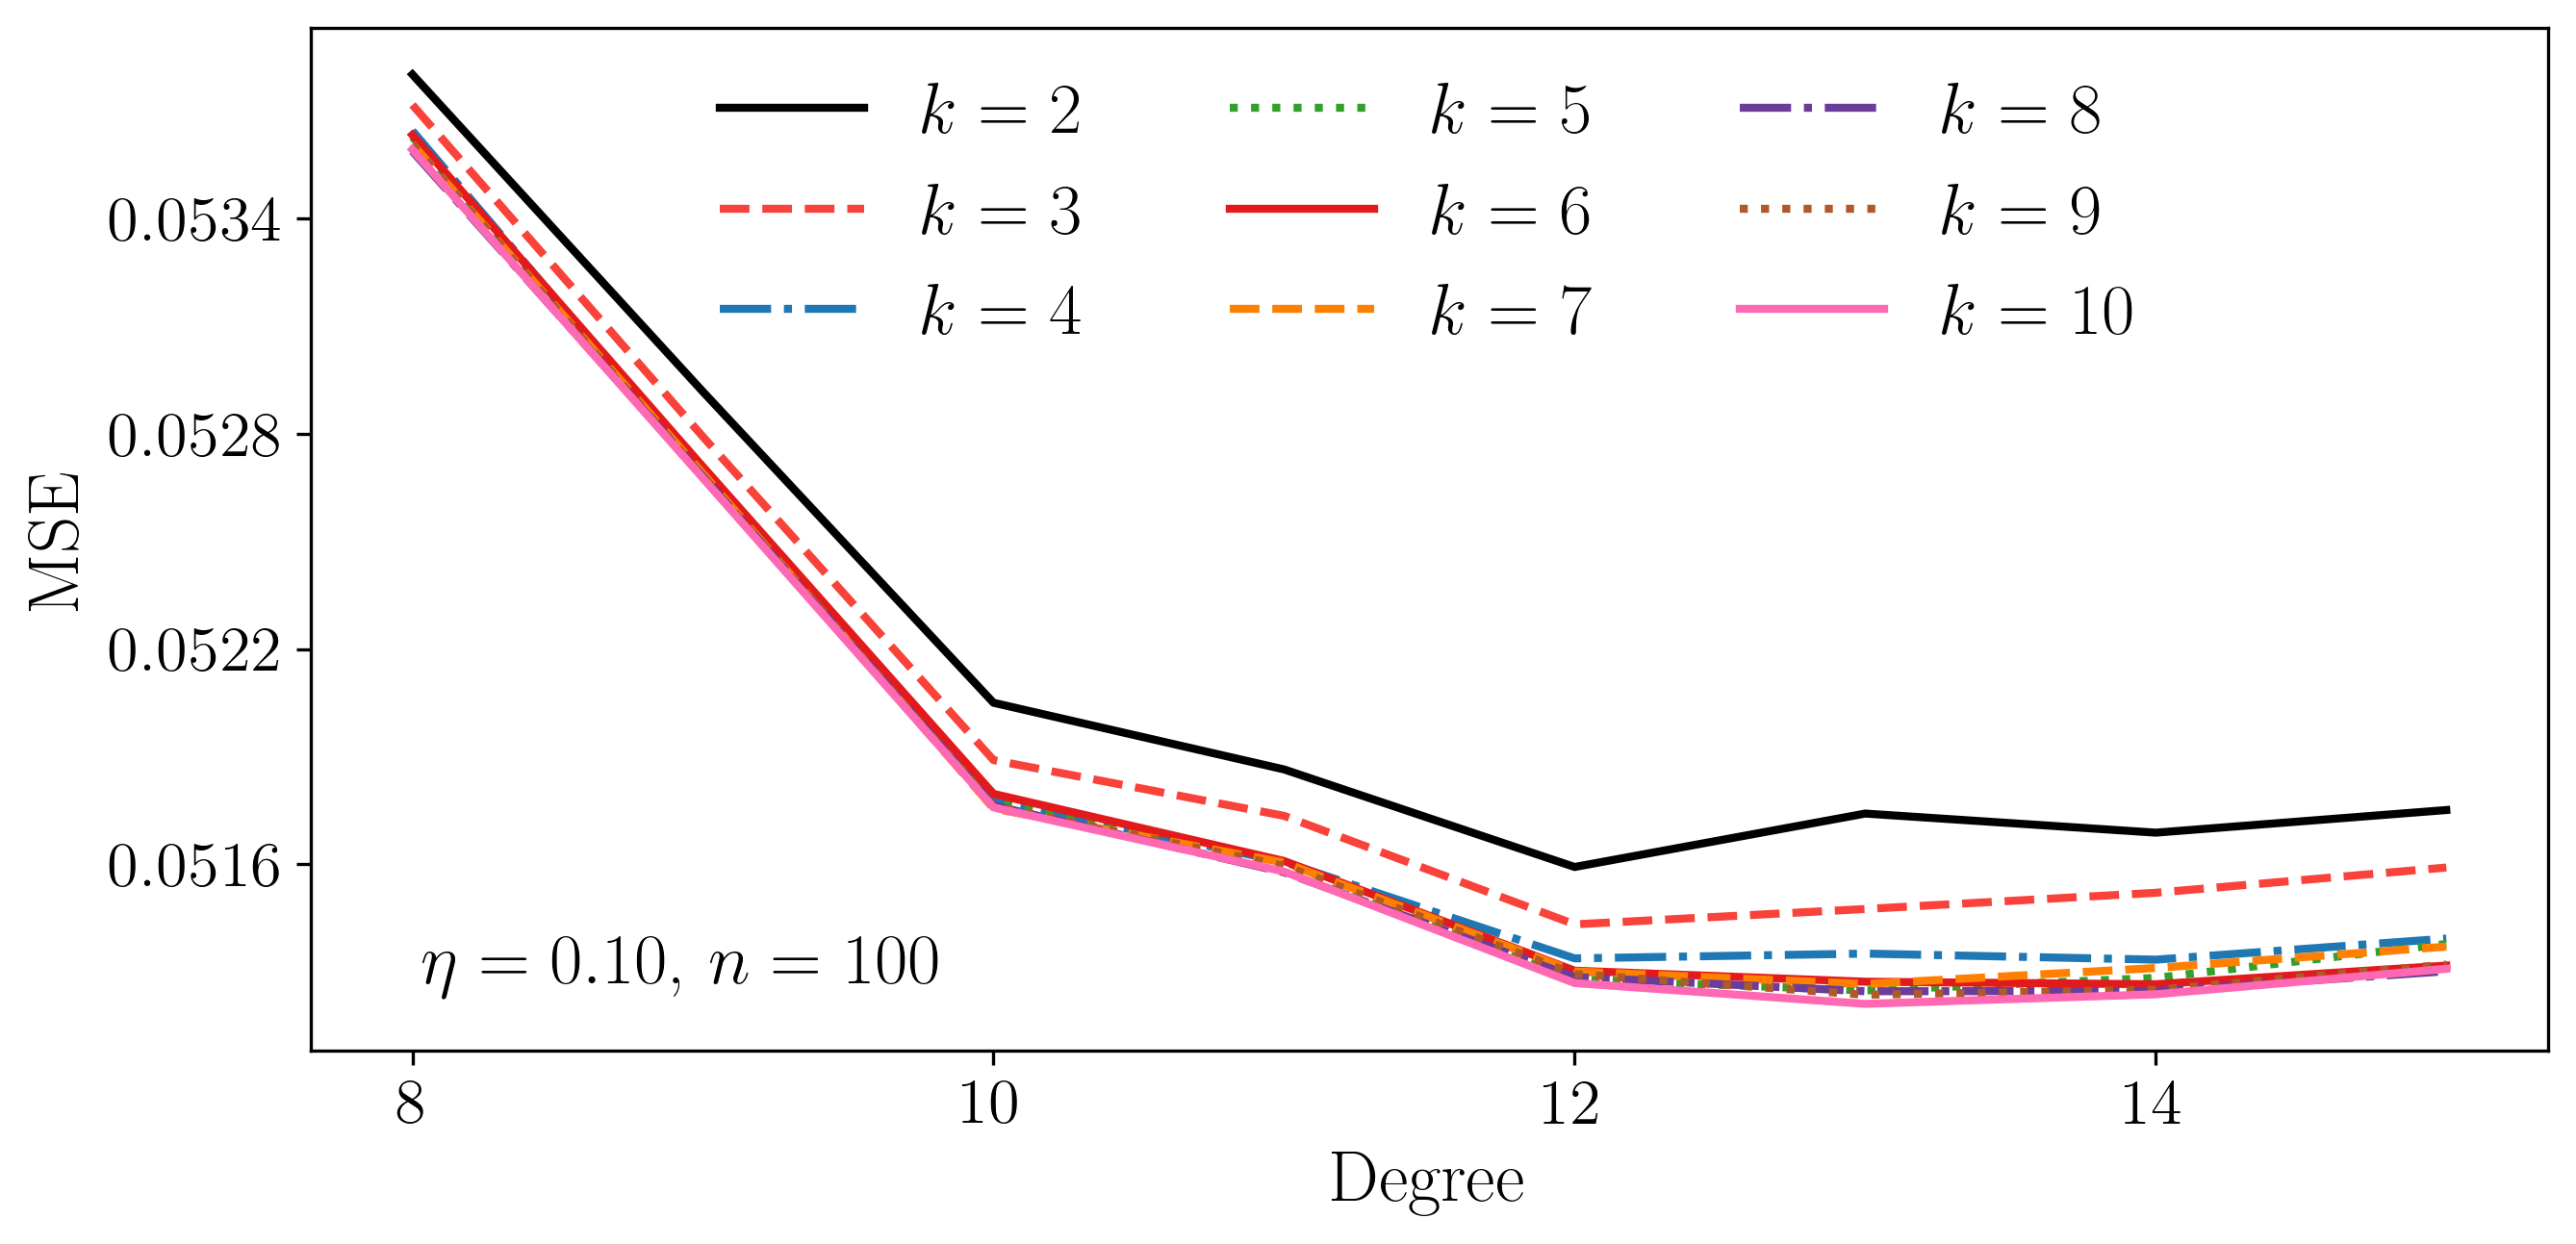
\includegraphics[width=\textwidth]{figures/hakon/kfolds_franke_15_k2_10.png}
        \end{minipage}
        \begin{minipage}{0.34\textwidth}
            \centering
            \textbf{F5} \label{fig:F5} \\  % Label added
            \includegraphics[width=\textwidth]{figures/hakon/betas_with_ci.png}
        \end{minipage}
        \begin{minipage}{0.32\textwidth}
            \centering
            \textbf{F6} \label{fig:F6} \\  % Label added
            \includegraphics[width=\textwidth]{figures/hakon/heatmap_ridge_4x4_minimal.png}
        \end{minipage}
        \hfill
        \begin{minipage}{0.32\textwidth}
            \centering
            \textbf{F7} \label{fig:F7} \\  % Label added
            \includegraphics[width=\textwidth]{figures/hakon/heatmap_lasso_4x4_minimal.png}
        \end{minipage}
        \begin{minipage}{0.34\textwidth}
            \centering
            \textbf{F8} \label{fig:F8} \\  % Label added
            \includegraphics[width=\textwidth]{figures/hakon/bootstrap_Ridge_d1-25.png}
        \end{minipage}
        \begin{minipage}{0.34\textwidth}
            \centering
            \textbf{F9} \label{fig:F9} \\  % Label added
            \includegraphics[width=\textwidth]{figures/hakon/r2_plot_best_model.png}
        \end{minipage}
        \hfill
        \begin{minipage}{0.32\textwidth}
            \centering
            \textbf{F10} \label{fig:F10} \\  % Label added
            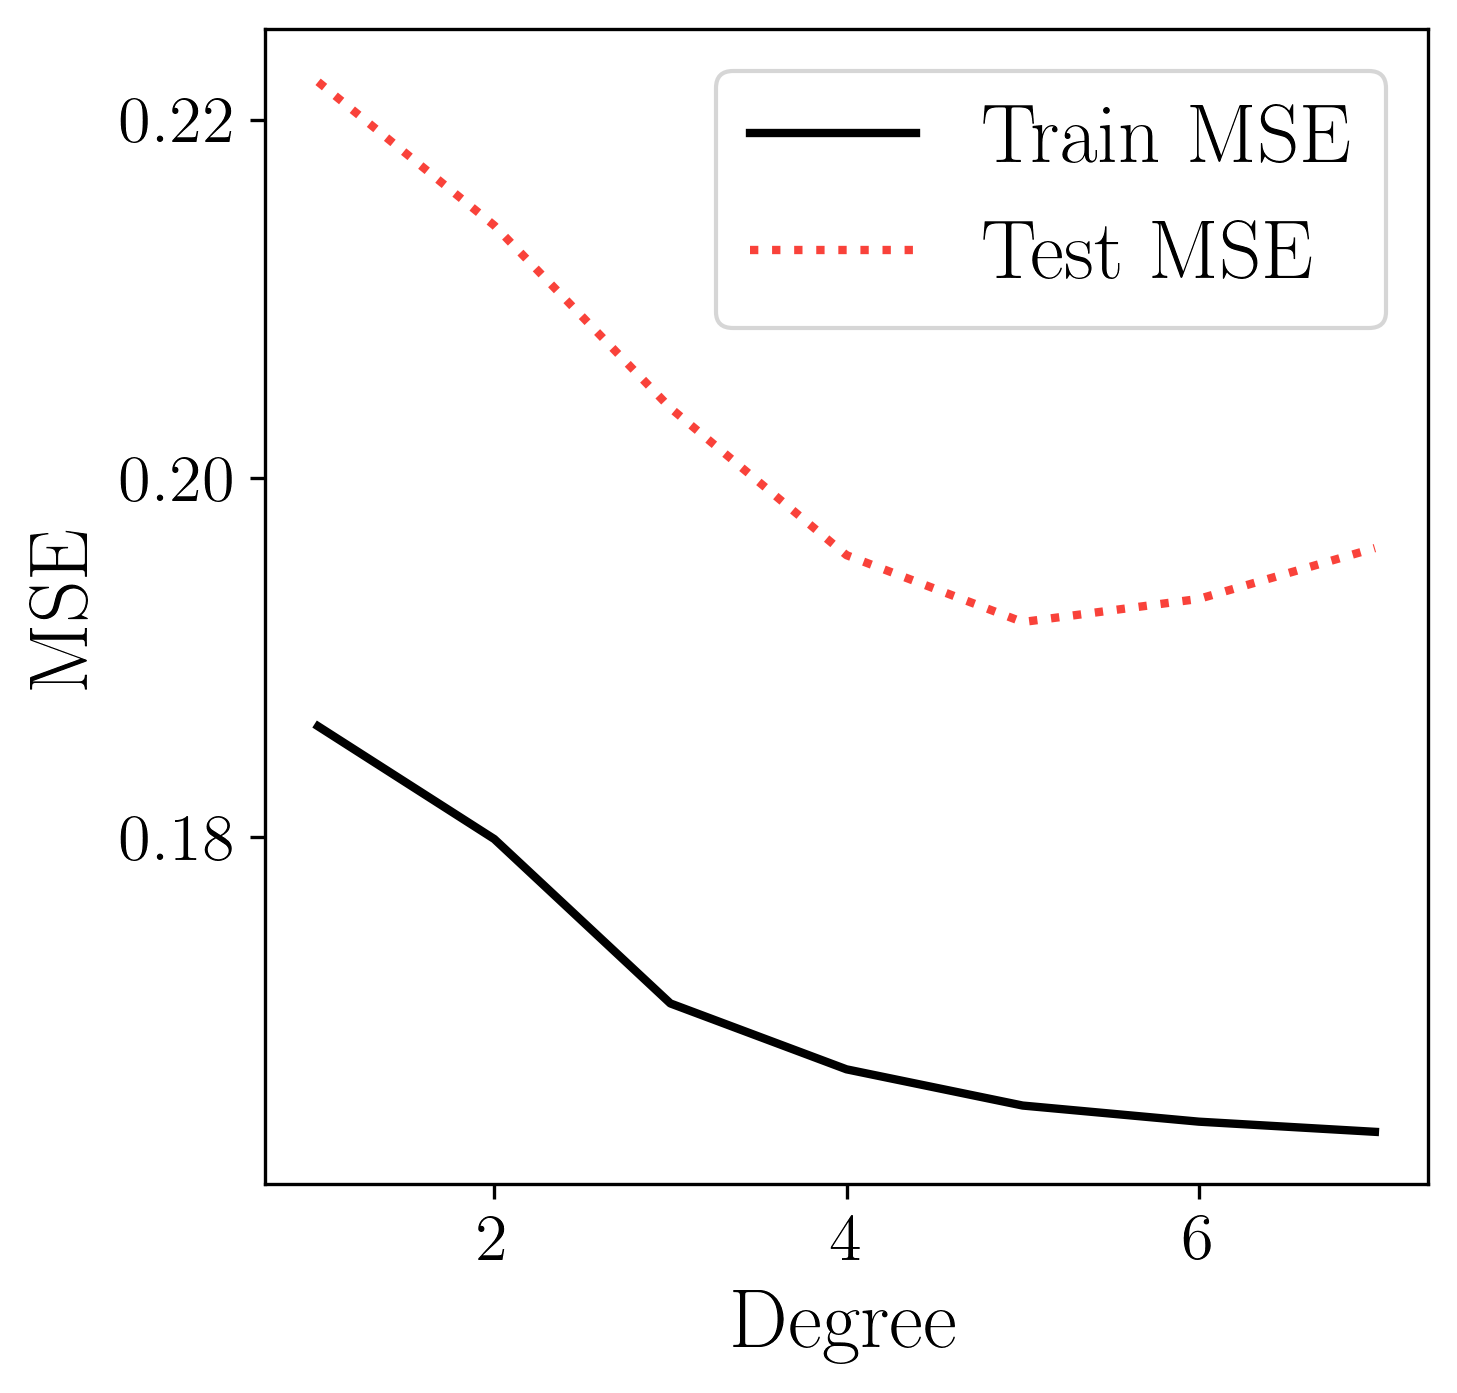
\includegraphics[width=\textwidth]{figures/hakon/train_test_plot_noise.png}
        \end{minipage}
        \begin{minipage}{0.32\textwidth}
            \centering
            \textbf{F11} \label{fig:F11} \\  % Label added
            \includegraphics[width=\textwidth]{figures/hakon/betas_of_lambda_ridge.png}
        \end{minipage}
             
        \vspace{1em}
        \caption*{\textbf{Plots from the testing of Franke’s function: }\textbf{F1} A visualisation of the terrain generated by Franke's function without noise, for $n=100$. \textbf{F2} The same function with added stochastic noise $\sim N(0, 1)$, $n =100, \eta = 0.10$. \textbf{F3} MSE for OLS regression as function of the degree of complexity, with and without the Singular Value Decomposition (SVD) as inversion-method. \textbf{F4} $k$-fold cross-validation, demonstrating that higher values of $k$ lead to more stable error estimates. $k = 10$ strikes a good balance between accuracy and computational efficiency. \textbf{F5} Coefficients with $\bm{\beta}$ with 95\% CI for degree 4 \textbf{F6} Heat maps for Ridge regression. The red frame indicates the lowest MSE at $0.01034$ for $\lambda=10^{-9}$ and polynomial degree = $18$. \textbf{F7} Heat map for lasso regression. Lowest MSE value $0.01433$ for $\lambda=10^{-7}$ and polynomial degree = $18$. \textbf{F8} Plot of bias-variance tradeoff for OLS with bootstrap. Bias and MSE stabilize around degree 6-10, with the MSE climbing again from around degree 18. \textbf{F9} Both OLS and Ridge regression achieve stable and high R$^2$-scores (around $90\%$) at polynomial degree $\sim6$. \textbf{F10} Train/test-plot for added noise $\sim N(0, 1),\ \eta=0.1$. Here we observed wrong values when using our own methods. \texttt{scikit learn}’s methods has been applied. We don’t see that this error affects any of the other analysis. \textbf{F11} Shrinkage plot of $\beta$-coefficients for increasing $\lambda$ in Ridge.} 
        \label{fig:franke_figs}
    \end{minipage}
    }
\end{figure}

%%%%%%%%%%%%%%%%%%%%%%%%%%%%%%%%%%%%%%%%%%%%%%%%%%%%%%%%
%                      TERRAIN                         %
%%%%%%%%%%%%%%%%%%%%%%%%%%%%%%%%%%%%%%%%%%%%%%%%%%%%%%%%

\section*{Testing with Real Terrain Data}

\begin{multicols}{2}
While Franke's function provides a good test case for evaluating our methods, it remains synthetic, and does not reflect the full complexity of real terrain. Having established that our methods work, they can be further applied. This will allow us to assess how well the best of our former parameters will work on new data, as well as fine-tune them further for improved accuracy in a more complex terrain. 

During the testing for Franke's function we have established that the bootstrap method works excellent for assessing a bias-variance tradeoff analysis, as well as the k-fold cross-validation method for assessing the MSE (We look here at $\sqrt{MSE}$, as this provides us with the error given in meters). We will analyze a $50\times 50$ section of the terrain illustrated in Figure \hyperref[fig:T1]{\textbf{T1}}, representing a complex mountainous region.

The terrain data is imported as a \texttt{.tif} file, which we convert into a 2D array using the \texttt{imageio} library in Python. Each pixel in the file has a resolution of 1 arc-second, approximately corresponding to 30 meters. Each entry in the array represents the height of a pixel in the selected area. Specifically, we extract data from the region defined by the coordinates $[200, 250]$ in both the $x$ and $y$ dimensions from the \texttt{stavanger.tif} file.

\subsubsection*{$k$-fold to assess error}
Figure \hyperref[fig:T2]{\textbf{T2}} presents a heatmap comparing real-world performance of Ridge regression (OLS included at $\lambda = 0$) and Lasso. For Franke's function we identify the optimal parameters through a L2-norm regularization. However when applying the same models to real-world terrain, the optimal parameters are found without regularization (i.e. OLS). Interestingly, we find that the same degree of complexity (degree = 18) minimizes both Franke's function and the real-world terrain. The minimal MSE for the terrain is found to be $3.669$ meters. We deem this to be a low MSE considering that we are examining a complex area. 

Despite that some regularization to Franke's function has shown improvement in MSE (for $\eta = 0.1$), we observe that OLS outperforms any means of regularization with the mountainous area. We propose that this could be due to the nature of a real terrain. Noise $\eta = 0.1$ in combination with Franke's function might not capture the nature of a real terrain. 

\subsection*{Bias-variance analysis for real terrain}
As discussed for Franke's function, analyzing performance using only $k$-fold cross-validation for MSE might not capture the full picture. Therefore, we also examine the bias-variance tradeoff for real terrain data. Once again, we employ the bootstrap method, as it proved to be a powerful method for analyzing Franke's function.

Figure \hyperref[fig:T3]{\textbf{T3}} shows the bias-variance tradeoff for OLS for real-terrain data.
By reducing the degree of complexity, we are able to reduce the variance significantly. By the eye analysis, shows that the best tradeoff lies in the range $[14, 17]$. So even though complexity 18 proved the lowest MSE for cross validation, it could be beneficial to reduce the complexity marginally to gain even more stable results. 

\section*{Conclusion}
In this project, we have explored the use of three different polynomial regression methods: Ordinary Least Squares (OLS), Ridge, and Lasso regression. Our analysis was conducted on both synthetic data generated by Franke’s function and real terrain data from a mountainous area outside Stavanger, Norway.

Our findings indicates that OLS outperforms both Ridge and Lasso in approximating the real world terrain. The best OLS model achieved a low $\sqrt{\text{MSE}}$ of $3.669$ meters.

While it may be tempting to choose the model with the lowest MSE, we also considered a bias-variance tradeoff. This led us to conclude that a model with less degree of complexity might provide more stable estimates. 

Given more time, we would conduct our analysis on multiple real-world terrains to develop a set of hyperparameters that could generalize well across a diverse range of landscapes.

Some final words: Although this has been a project in machine learning, it has involved quite a bit of \textbf{human learning}, too. We are three bachelor students who have now written our first research paper. It has been a steep uphill journey of valuable learning and great collaboration. Now, our hyperparameters are tuned, and our brains’ models on paper-writing are trained, and we feel very ready to tackle a new assignment.
\end{multicols}

\begin{figure}[H]
    \centering
    \fbox{
    \begin{minipage}{\textwidth}
        \centering
        \begin{minipage}{0.32\textwidth}
            \centering
            \textbf{T1} \label{fig:T1} \\  % Label added
            \includegraphics[width=\textwidth]{figures/hakon/terrain.png}
        \end{minipage}
        \hfill
        \begin{minipage}{0.32\textwidth}
            \centering
            \textbf{T2} \label{fig:T2} \\  % Label added
            \includegraphics[width=\textwidth]{figures/hakon/terr_heatmap_ridge_4x4_minimal.png}
        \end{minipage}
        \hfill
        \begin{minipage}{0.32\textwidth}
            \centering
            \textbf{T3} \label{fig:T3} \\  % Label added
            \includegraphics[width=\textwidth]{figures/hakon/terr_heatmap_lasso_4x4_minimal.png}
        \end{minipage}
        \begin{minipage}{\textwidth}
            \centering
            \textbf{T4} \label{fig:T4} \\  % Label added
            \includegraphics[width=0.40\textwidth]{figures/hakon/terr_bootstrap_Ridge_d1-25.png}
        \end{minipage}
        \begin{minipage}{0.49\textwidth}
            \centering
            \textbf{T5} \label{fig:T5} \\  % Label added
            \includegraphics[width=\textwidth]{figures/hakon/real_terr.png}
        \end{minipage}
        \hfill
        \begin{minipage}{0.49\textwidth}
            \centering
            \textbf{T6} \label{fig:T6} \\  % Label added
            \includegraphics[width=\textwidth]{figures/hakon/terr_Ridge_deg16_lmd0_no_int.png}
        \end{minipage}
        
        \vspace{1em}
        \caption*{\textbf{Plots from the testing of real terrain from Evje, outside Stavanger: }\textbf{T1} Plot of the $50 \times 50$ terrain grid, representing a complex mountainous region. \textbf{T2} Heat map of Ridge/OLS regression MSEs for increasing regularization term $\lambda$ and polynomial degree for the same terrain. The red square indicates the lowest MSE for Degree 18. This shows that OLS yields the best result in our model, with a $\sqrt{\text{MSE}}$ of 3.669 meters. \textbf{T3} Heat map of Lasso MSEs for increasing $\lambda$ and degree. The red square indicates the lowest MSE for Degree 28. This shows that Lasso is unable to outperform OLS, with a $\sqrt{\text{MSE}}$ of 14.640 meters. \textbf{T4} Bias-variance tradeoff plot for OLS for the terrain data. Visual inspection indicates best tradeoff can be found between polynomial degrees $[14-17]$. \textbf{T5} 3D-visualization of the \textit{real} landscape in figure T1. \textbf{T6} Visualization of the modelled landscape, with the chosen model and hyper parameters tuned: OLS with $\text{degree} = 16$, which is in accordance with our bias-variance tradeoff findings (T3).}
        \label{fig:terr_figs}
    \end{minipage}
    }
\end{figure}
\bibliographystyle{unsrt}
\bibliography{references}
\newpage

%%%%%%%%%%%%%%%%%%%%%%%%%%%%%%%%%%%%%%%%%%%%%%%%%%%%%%%%
%                     APPENDIX                         %
%%%%%%%%%%%%%%%%%%%%%%%%%%%%%%%%%%%%%%%%%%%%%%%%%%%%%%%%

\appendix
\section*{Appendix}
\noindent \textbf{Regression Analysis and Resampling Techniques in Applied Machine Learning}

% Appendix A
\section{Algorithms}
\label{app:something}
\subsection{Design matrix setup - Pseudocode}
\label{app_alg:design_matrix}
We set up the design matrix with the following algorithm:
\lstset{
    language=Python,         % Specify the language for syntax highlighting (e.g., Python, C++, Java)
    basicstyle=\ttfamily,    % Set font to monospace
    keywordstyle=\color{blue}, % Customize keyword color
    commentstyle=\color{gray},  % Customize comment color
    stringstyle=\color{red},   % Customize string color
    breaklines=true           % Enable line breaking
}
\begin{lstlisting}
    idx = 0
    for i in range(degree+1):
        for j in range(degree+1): 
            if i+j <= degree:
                entry = (x**i * y**j)
                X[:, idx] = entry
                idx += 1
\end{lstlisting}

\section{Preprocessing steps}
\label{app:dataset}
\subsection{A note on the Intercept}
\label{app_prep:intercept}
In a standard polynomial regression analysis, the first coefficient, $\bm{\beta}_0$ is always multiplied by $1$, eliminating the dependency on the variable $\bm{x}$. As a result, when all predictors are set to zero, $\bm{\beta}_0$ becomes the sole predictor, denoted as the \texttt{intercept}.

A common approach is to include the intercept in the \texttt{design\_matrix} as a column of $1s$. This ensures that the regression model fits the intercept during training. Alternatively, the intercept can be excluded during training, and calculated afterwards using the this equation:

$$\beta_0 = \frac{1}{n}\sum_{i=0}^{n-1}y_i - \sum_{j=1}^{p-1} \mu_{\boldsymbol{x}_j}\beta_j$$

For OLS regression, the disticinton is marginal. However, in Ridge and Lasso regression, exclucing the intercept from the regularization term, can make a more significant difference.

\section{Resampling techniques}
\label{app:resampling}
\subsection{The bootstrap algorithm}
\label{app_resamp:bootstrap}
The \textbf{algorithm} is as follows:

\begin{enumerate}
    \item \textbf{Initialize:} Given a dataset $D = \{x_0, x_1, \ldots, x_{n-1}\}$, choose the number of bootstrap iterations \texttt{B}.
    \item \textbf{Resample:} For each bootstrap iteration $b = 1, 2, \dots, B$:
    \begin{itemize}
        \item Randomly draw a sample of size $n$ from $D$, with replacement, to form a resampled dataset $D_b$.
        \item Compute the desired statistic $\hat{\theta}_b$ using $D_b$.
    \end{itemize}
    \item \textbf{Estimate:} After $B$ iterations, calculate the final estimate of the statistic as the average of $\hat{\theta}_b$:
    \[
    \hat{\theta}_{\text{bootstrap}} = \frac{1}{B} \sum_{b=0}^{B-1} \hat{\theta}_b
    \]
\end{enumerate}

% Appendix B
\section{Mathematical Derivations}
\label{app:derivations}

\subsection{Optimal coefficients for OLS}
\label{app_derivations:beta_ols_without_svd}
To show that the optimal coefficients $\hat{\beta}$ for OLS regression is 
$$\bm{\hat{\beta}} = (\mathbf{X}^{T}\mathbf{X})^{-1}\mathbf{X}^{T}\bm{z}$$ 
we can minimize the following cost-function
$$C(\mathbf{X}, \bm{\beta}) = \{(\bm{z} - \mathbf{X}\bm{\beta})^{T}(\bm{z} - \mathbf{X}\bm{\beta})\}$$
We can rewrite $C(\mathbf{X}, \bm{\beta})$ to 
$$C(\mathbf{X}, \bm{\beta}) = \bm{z}^{T}\bm{z} - \bm{z}^{T}\mathbf{X}\bm{\beta} - \bm{\beta}^{T}\mathbf{X}^{T}\bm{z} + \bm{\beta}^{T}\mathbf{X}^{T}\mathbf{X}\bm{\beta}$$
We have that
\begin{align} \label{eq:OLS_appendix}
    (\bm{z}^{T}\mathbf{X}\bm{\beta})^{T} = \bm{\beta}^{T}\mathbf{X}^{T}\bm{z}  
\end{align}
And since \ref{eq:OLS_appendix} is a scaler we have that the transpose of \ref{eq:OLS_appendix} is itself. \\
We can therefore rewrite $C(\mathbf{X}, \bm{\beta})$ to
$$C(\mathbf{X}, \bm{\beta}) = \bm{z}^{T}\bm{z} - 2\bm{\beta}^{T}\mathbf{X}^{T}\bm{z} + \bm{\beta}^{T}\mathbf{X}^{T}\mathbf{X}\bm{\beta}$$
We can now optimize $C(\mathbf{X}, \bm{\beta})$, we can do this by setting $\frac{\partial C(\mathbf{X}, \bm{\beta})}{\partial \bm{\beta}} = 0.$
\begin{align*}
    \frac{\partial C(\mathbf{X}, \bm{\beta})}{\partial \bm{\beta}} &= -2\frac{\partial}{\partial\bm{\beta}}  \bm{\beta}^{T}\mathbf{X}^{T}\bm{z} +  \frac{\partial}{\partial \bm{\beta}} \bm{\beta}^{T}\mathbf{X}^{T}\mathbf{X}\bm{\beta} \\
    &= -2\bm{z}^{T}\mathbf{X} + 2\bm{\beta}^{T}\mathbf{X}^{T}\mathbf{X} 
\end{align*}
Setting this equal to zero yields
\begin{align*}
    \bm{z}^{T}\mathbf{X} - \bm{\beta}^{T}\mathbf{X}^{T}\mathbf{X} = 0
\end{align*}
This rewrites to
$$\bm{\hat{\beta}} = (\mathbf{X}^{T}\mathbf{X})^{-1}\mathbf{X}^{T}\bm{z}$$ 

\subsection{Optimal coefficients for Ridge}
\label{app_derivations:beta_ridge_without_svd}
To show that the optimal parameters $\hat{\beta}$ for 
ridge regression is 
$$\bm{\hat{\beta}} = (\mathbf{X}^{T}\mathbf{X} + \lambda\mathbf{I})^{-1}\mathbf{X}^{T}\bm{z}$$ 
we can minimize the following cost-function
$$C(\mathbf{X}, \bm{\beta}) = \{(\bm{z} - \mathbf{X}\bm{\beta})^{T}(\bm{z} - \mathbf{X}\bm{\beta})\} + \lambda\bm{\beta}^{T}\bm{\beta}$$
We can rewrite $C(\mathbf{X}, \bm{\beta})$ to 
$$C(\mathbf{X}, \bm{\beta}) = \bm{z}^{T}\bm{z} - \bm{z}^{T}\mathbf{X}\bm{\beta} - \bm{\beta}^{T}\mathbf{X}^{T}\bm{z} + \bm{\beta}^{T}\mathbf{X}^{T}\mathbf{X}\bm{\beta} + \lambda\bm{\beta}^{T}\bm{\beta}$$
We have that
\begin{align} \label{eq:Ridge_appendix}
    (\bm{z}^{T}\mathbf{X}\bm{\beta})^{T} = \bm{\beta}^{T}\mathbf{X}^{T}\bm{z}  
\end{align}
And since \ref{eq:Ridge_appendix} is a scaler we have that the transpose of \ref{eq:Ridge_appendix} is itself. \\
We can therefore rewrite $C(\mathbf{X}, \bm{\beta})$ to
$$C(\mathbf{X}, \bm{\beta}) = \bm{z}^{T}\bm{z} - 2\bm{\beta}^{T}\mathbf{X}^{T}\bm{z} + \bm{\beta}^{T}\mathbf{X}^{T}\mathbf{X}\bm{\beta} + \lambda\bm{\beta}^{T}\bm{\beta}$$
We can now optimize $C(\mathbf{X}, \bm{\beta})$, we can do this by setting $\frac{\partial C(\mathbf{X}, \bm{\beta})}{\partial \bm{\beta}} = 0.$
\begin{align*}
    \frac{\partial C(\mathbf{X}, \bm{\beta})}{\partial \bm{\beta}} &= -2\frac{\partial}{\partial\bm{\beta}}  \bm{\beta}^{T}\mathbf{X}^{T}\bm{z} +  \frac{\partial}{\partial \bm{\beta}} \bm{\beta}^{T}\mathbf{X}^{T}\mathbf{X}\bm{\beta} + \lambda \frac{\partial}{\partial \bm{\beta}} \bm{\beta}^T\bm{\beta} \\
    &= -2\bm{z}^{T}\mathbf{X} + 2\bm{\beta}^{T}\mathbf{X}^{T}\mathbf{X} + 2 \lambda \bm{\beta}^{T}
\end{align*}
Setting this equal to zero yields
\begin{align*}
    \bm{z}^{T}\mathbf{X} - \bm{\beta}^{T}\mathbf{X}^{T}\mathbf{X} - \lambda \bm{\beta}^{T} = 0
\end{align*}
This rewrites to
$$\bm{\hat{\beta}} = (\mathbf{X}^{T}\mathbf{X} + \lambda\mathbf{I})^{-1}\mathbf{X}^{T}\bm{z}$$ 

\subsection{Optimal predicts using OLS with SVD approach}
\label{app_derivations:predicts_ols_with_svd}
To show that we can write the OLS solutions in terms of the eigenvectors of the orthogonal matrix $\mathbf{U}$ as
$$\bm{\tilde{z}}_{OLS} = \mathbf{X}\bm{\beta}_{OLS} = \sum_{j=0}^{p-1}\bm{u}_{j}\bm{u}_{j}^{T}\bm{z}$$
We can start with the OLS equation and combine it with the singular value decomposition, meaning
\begin{align*}
    \bm{\tilde{z}}_{OLS} = \mathbf{X}\bm{\beta} &= \mathbf{X}(\mathbf{X}^{T}\mathbf{X})^{-1}\mathbf{X}^{T}\bm{z} \\
    \mathbf{X} &= \mathbf{U}\bm{\Sigma}\mathbf{V}^{T}
\end{align*}
Combining these yields
\begin{align*}
    &= \mathbf{U}\bm{\Sigma}\mathbf{V}^{T}(\mathbf{V}\bm{\tilde{{\Sigma}}}^{2}\mathbf{V}^{T})^{-1}\mathbf{V}\mathbf{\Sigma}^{T}\mathbf{U}^{T}\bm{z} \\
    &= \mathbf{U}\bm{\Sigma}\mathbf{V}^{T}\mathbf{V}(\bm{\tilde{{\Sigma}}}^{2})^{-1}\mathbf{V}^{T}\mathbf{V}\mathbf{\Sigma}^{T}\mathbf{U}^{T}\bm{z} \\ 
    &= \mathbf{U}\bm{\Sigma}(\bm{\tilde{{\Sigma}}}^{2})^{-1}\mathbf{\Sigma}^{T}\mathbf{U}^{T}\bm{z} \\
\end{align*}
The expression $\bm{\Sigma}(\bm{\tilde{{\Sigma}}}^{2})^{-1}\mathbf{\Sigma}^{T}$ is a matrix with the same dimensions as $\bm{\Sigma}$.
If $\bm{\Sigma}$ has p singular values then $\bm{\Sigma}(\bm{\tilde{{\Sigma}}}^{2})^{-1}\mathbf{\Sigma}^{T}$ has p ones along the
diagonal, and n-p zero columns.  
This gives 
$$\bm{\tilde{z}}_{OLS} = \mathbf{U}\mathbf{U}^{T}\bm{z} = \sum_{j=0}^{p-1}\bm{u}_{j}\bm{u}_{j}^{T}\bm{z}$$

\subsection{Optimal coefficients using OLS with SVD approach}
\label{app_derivations:beta_ols_with_svd}
Under follows the full derivation for the optimal OLS coefficients, here we have used the SVD approch:
\begin{align*}
    \bm{\hat{\beta}}_\text{OLS} &= (\XX^\top\XX)^{-1}\XX^\top\bm{z} \\
    &=(\VV\mathbf{\Sigma}^\top\UU^\top\UU\mathbf{\Sigma}\VV^\top)^{-1}\VV\mathbf{\Sigma}^\top\UU^\top\bm{z} \\
    &= (\VV\mathbf{\Sigma}^\top\mathbf{\Sigma}\VV^\top)^{-1}\VV\mathbf{\Sigma}^\top\UU^\top\bm{z} \\
    &= \VV(\mathbf{\Sigma}^\top\mathbf{\Sigma})^{-1}\VV^\top\VV\mathbf{\Sigma}^\top\UU^\top\bm{z} \\
    &= \VV(\mathbf{\Sigma}^\top\mathbf{\Sigma})^{-1}\mathbf{\Sigma}^\top\UU^\top\bm{z} 
\end{align*}

\subsection{Optimal predicts using Ridge regression with SVD approach}
\label{app_derivations:predicts_ridge_with_svd}
For Ridge regression we want to show that the corresponsing equation is
$$\bm{\tilde{z}}_{Ridge} = \mathbf{X}\bm{\beta}_{Ridge} = \sum_{j=0}^{p-1}\bm{u}_{j}\bm{u}_{j}^{T} \frac{\sigma_{j}^{2}}{\sigma_{j}^2 + \lambda} \bm{z}$$
We start with the optimized cost-function for Ridge and combine it with SVD. 
\begin{align*}
    \bm{\tilde{z}}_{Ridge} &= \mathbf{X}\bm{\beta}_{Ridge} = \mathbf{X}(\mathbf{X}^{T}\mathbf{X} + \lambda\mathbf{I})^{-1}\mathbf{X}^{T}\bm{z} \\
    \mathbf{X} &= \mathbf{U}\bm{\Sigma}\mathbf{V}^{T}
\end{align*}
Combining these yields
\begin{align*}
    \bm{\tilde{z}}_{Ridge} &= \mathbf{U}\bm{\Sigma}\mathbf{V}^{T}(\mathbf{V}\bm{\Sigma}^{T}\mathbf{U}^{T}\mathbf{U}\bm{\Sigma}\mathbf{V}^{T} + \mathbf{I}\lambda)^{-1}\mathbf{V}\mathbf{\Sigma}^{T}\mathbf{U}^{T}\bm{z} \\
    &= \mathbf{U}\bm{\Sigma}\mathbf{V}^{T}(\mathbf{V}\bm{\Sigma}^{T}\bm{\Sigma}\mathbf{V}^{T} + \mathbf{I}\lambda)^{-1}\mathbf{V}\mathbf{\Sigma}^{T}\mathbf{U}^{T}\bm{z} \\ 
    &= \mathbf{U}\bm{\Sigma}\mathbf{V}^{T}(\mathbf{V}\bm{\tilde{\Sigma}}^{2}\mathbf{V}^{T} + \mathbf{I}\lambda)^{-1}\mathbf{V}\mathbf{\Sigma}^{T}\mathbf{U}^{T}\bm{z} \\
    &= \mathbf{U}\bm{\Sigma}\mathbf{V}^{T}(\mathbf{V}\bm{\tilde{\Sigma}}^{2}\mathbf{V}^{T} + \lambda\mathbf{V}\mathbf{V}^{T})^{-1}\mathbf{V}\mathbf{\Sigma}^{T}\mathbf{U}^{T}\bm{z} \\
    &= \mathbf{U}\bm{\Sigma}\mathbf{V}^{T}(\mathbf{V}(\bm{\tilde{\Sigma}}^{2} + \lambda\mathbf{I})\mathbf{V}^{T})^{-1}\mathbf{V}\mathbf{\Sigma}^{T}\mathbf{U}^{T}\bm{z} \\
    &= \mathbf{U}\bm{\Sigma}\mathbf{V}^{T}\mathbf{V}(\bm{\tilde{\Sigma}}^{2} + \lambda\mathbf{I})^{-1}\mathbf{V}^{T}\mathbf{V}\mathbf{\Sigma}^{T}\mathbf{U}^{T}\bm{z} \\
    &= \mathbf{U}\bm{\Sigma}(\bm{\tilde{\Sigma}}^{2} + \lambda\mathbf{I})^{-1}\mathbf{\Sigma}\mathbf{U}^{T}\bm{z} \\
\end{align*} 
$\bm{\Sigma}(\bm{\tilde{\Sigma}}^{2} + \lambda\mathbf{I})^{-1}\bm{\Sigma}$ is the same situation as for OLS, but
instead of ones along the diagonal we get $\frac{\sigma_{j}^{2}}{\sigma_{j}^2 + \lambda}$ along the diagonal. 
In total we therefor have
$$\bm{\tilde{z}}_{Ridge} = \sum_{j=0}^{p-1}\bm{u}_{j}\bm{u}_{j}^{T} \frac{\sigma_{j}^{2}}{\sigma_{j}^2 + \lambda} \bm{z}$$



\subsection{Optimal coefficients using Ridge regression with SVD approach}
\label{app_derivations:beta_ridge_with_svd}
Under follows the full derivation for the optimal Ridge coefficients, here we have used the SVD approch:
\begin{align*}
    \bm{\hat{\beta}}_\text{Ridge} &= 
    (\XX^\top\XX + \lambda I)^{-1}\XX^\top\bm{z} \\
    &=
    (\VV\mathbf{\Sigma}^\top\UU^\top\UU\mathbf{\Sigma}\VV^\top+\lambda I)^{-1}\VV\mathbf{\Sigma}^\top\UU^\top\bm{z} \\
    &=
    (\VV\mathbf{\Sigma}^\top\mathbf{\Sigma}\VV^\top+\lambda I)^{-1}\VV\mathbf{\Sigma}^\top\UU^\top\bm{z} \\
    &=
    (\VV\mathbf{\Sigma}^\top\mathbf{\Sigma}\VV^\top+\VV\lambda \VV^\top)^{-1}\VV\mathbf{\Sigma}^\top\UU^\top\bm{z} \\
    &=
    (\VV(\mathbf{\Sigma}^\top\mathbf{\Sigma}\ + \lambda I) \VV^\top)^{-1}\VV\mathbf{\Sigma}^\top\UU^\top\bm{z} \\
    &=
    \VV(\mathbf{\Sigma}^\top\mathbf{\Sigma}\ + \lambda I)^{-1} \VV^\top\VV\mathbf{\Sigma}^\top\UU^\top\bm{z} \\
    &=
    \VV(\mathbf{\Sigma}^\top\mathbf{\Sigma}\ + \lambda I)^{-1} \mathbf{\Sigma}^\top\UU^\top\bm{z} 
\end{align*}

\subsection{Expectation and Variance of the True Response Function}
\label{app_derivations:expectation_variance_true_z}
We can further understand the behaviour of $\bm{z} = f(\bm{x}) + \epsilon$ by looking at its expectation and variance. We first look at the expectation:
\begin{align*}
    \EE[z_i] &= \EE[f(\bm{x}_i) + \epsilon_i] \\
    &= \EE[f(\bm{x}_i)] + \EE[\epsilon_i] 
\end{align*}
$f(\bm{x}_i)$ is non-stochastic and $\epsilon \sim \mathcal{N}(0, \sigma^2)$
In total we therefore have
$$\EE[z_i] = f(\bm{x}_i) = \sum_{j} x_{ij}\beta_j = \mathbf{X}_{i, *}\bm{\beta}$$
Now the variance:
\begin{align*}
    \text{Var}[z_i] &= \EE[z_{i}^2] - \EE[z_i]^2 \\
    &= \EE[f(\bm{x}_i + \epsilon_i)^2] - f(\bm{x}_i)^2 \\
    &= \EE[f(\bm{x}_i)^2] + \EE[\epsilon_{i}^{2}] + \EE[2f(\bm{x}_i)\epsilon_i] - f(\bm{x}_i)^2 \\
    &= f(\bm{x}_i)^2 + \EE[\epsilon_i^2] - f(\bm{x}_i)^2 \\
    &= \EE[\epsilon_i^2] = \text{Var}[\epsilon_i] + \EE[\epsilon_i]^2 \\
    &= \sigma^2
\end{align*}


\subsection{Expectation for beta and variance for OLS}
\label{app_derivations:expectation_variance_betas}
We want to show that $\EE[\hat{\bm{\beta}}] = \bm{\beta}$. This can be done with the following reasoning:
\begin{align*}
    \EE[\hat{\bm{\beta}}] &= \EE[(\mathbf{X}^\top\mathbf{X})^{-1}\mathbf{X}^\top \bm{z})] \\
    &= (\mathbf{X}^\top\mathbf{X})^{-1}\mathbf{X}^\top \EE[\bm{z}] \\
    &= (\mathbf{X}^\top\mathbf{X})^{-1}\mathbf{X}^\top \mathbf{X} \bm{\beta} \\
    &= \bm{\beta}
\end{align*}
Further we want to show that $\text{Var}[\hat{\bm{\beta}}] = \sigma^2(\mathbf{X}^\top\mathbf{X})^{-1}$. This can be done in the following derivation: 
$$\text{Var}[\hat{\bm{\beta}}] = \text{Var}[(\mathbf{X}^\top\mathbf{X})^{-1}\mathbf{X}^\top \bm{z})]$$
Set 
$$\text{H} = (\mathbf{X}^\top\mathbf{X})^{-1}\mathbf{X}^\top$$
We now use the follwoing identity 
$$\text{Var}[H\bm{z}] = H \text{Var}[\bm{z}]H^\top$$
Where $\text{Var}[\bm{z}] = \sigma^2$
We therefore have
$$\text{Var}[H\bm{z}] = \sigma^2 HH^\top$$
$HH^\top$ can be rewritten
\begin{align*}
    HH^\top &= (\mathbf{X}^\top\mathbf{X})^{-1}\mathbf{X}^\top \mathbf{X}((\mathbf{X}^\top\mathbf{X})^{-1})^\top \\
    &= ((\mathbf{X}^\top\mathbf{X})^{-1})^\top \\
    &= (\mathbf{X}^\top\mathbf{X})^{-1}
\end{align*}
In total we have therefore shown that
$$\text{Var}[\hat{\bm{\beta}}] = \sigma^2(\mathbf{X}^\top\mathbf{X})^{-1}$$


\subsection{Bias-variance decomposition}
\label{app_derivations:bias_variance_decomp}
We want to show that MSE can be rewritten as follows 
$$\EE[(\bb{z} - \tilde{\bb{z}})^{2}] = \text{Bias}[\tilde{\bb{z}}] + \text{Var}[\tilde{\bb{z}}] + \sigma^{2}$$
We can expand the MSE  
\begin{align*}
    \EE[(\bb{z} - \tilde{\bb{z}})^{2}] &= \EE[(\bb{z}^{2} + \tilde{\bb{z}}^{2} - 2\bb{z}\tilde{\bb{z}})] \\ 
    &= \EE[\bb{z}^{2}] + \EE[\ty^{2}] - 2\EE[\bb{z}\ty]
\end{align*}
We will now rewrite each term, first $\EE[\bb{z^2}]$
\begin{align*}
    \EE[\bb{z^2}] &= \text{Var}[\bb{z}] + \EE[\bb{z}]^{2} \\
    &= \text{Var}[f + \bb{\epsilon}] + \EE[f + \bb{\epsilon}]^{2} \\
    &= \text{Var}[f]+ \text{Var}[\bb{\epsilon}] + (\EE[f] + \EE[\epsilon])^{2} \\
    &= \sigma^{2}+ f^{2}
\end{align*}
Second $\EE[\ty^{2}]$
$$\EE[\ty^{2}] = \text{Var}[\ty] + \EE[\ty]^{2}$$
Last $\EE[\bb{z}\ty]$ 
\begin{align*}
    \EE[\bb{z}\ty] &= \EE[(f + \bb{\epsilon})\ty] \\
    &= \EE[f\ty + \bb{\epsilon}\ty] \\
    &= f\EE[\ty] + \EE[{\bb{\epsilon}}]\EE[\ty] \\
    &= f\EE[\ty]
\end{align*}
Putting it all together we have
\begin{align*}
    \EE[(\bb{z} - \tilde{\bb{z}})^{2}] &= \sigma^{2}+f^{2}+\text{Var}[\ty] + \EE[\ty]^{2} - 2f\EE[\ty] \\
    &= \sigma^{2} + \text{Var}[\ty] + f^{2} + \EE[\ty]^{2} - 2f\EE[\ty] \\
    &= \sigma^{2} + \text{Var}[\ty] + (f - \EE[\ty])^{2}
\end{align*}
Where the last term is the bias squared, often just called bias (it will always be positive). In total we therefore have
$$\EE[(\bb{z} - \tilde{\bb{y}})^{2}] = \text{Bias}[\tilde{\bb{z}}] + \text{Var}[\tilde{\bb{z}}] + \sigma^{2}$$

In practice, the true function $\bm{f}$ is generally unknown. As a consequence, we must replace $\bm{f}$ with the observed response $\bm{z}$ which incorporates the noise $\boldsymbol{\epsilon}$. This allows us to estimate bias and variance using the available data, though it introduces additional uncertainty due to the noise that comes included with $\bm{z}$.

\end{document}